\begin{figure}[p]
\centering
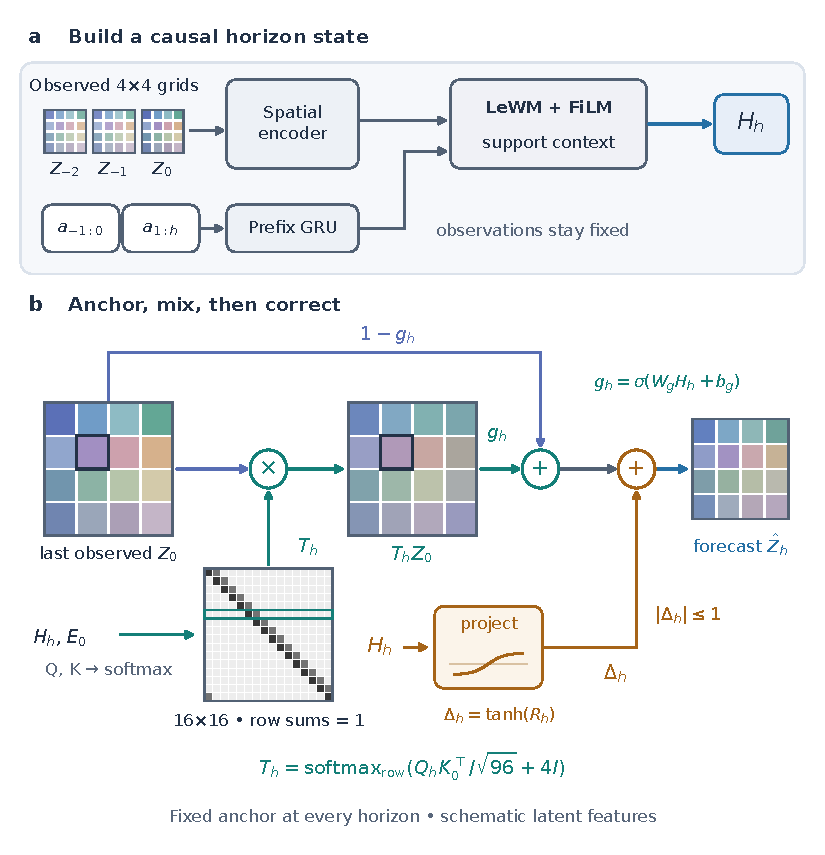
\includegraphics[width=\linewidth]{generated/real_video/spatial_method.pdf}
\caption{\textbf{Observation-anchored spatial candidate (ours), transport arm.}
(a) Three observed feature grids, support-only context and a causal action prefix produce horizon state $H_h$.
(b) The last observed grid $Z_0$ stays fixed at every horizon. Queries project $H_h$; keys project $E_0$, the last observed grid's spatial encoding \emph{before} context FiLM.
Row-stochastic weights mix semantic patch features, a sigmoid gate with explicit affine bias $b_g$ blends them with the anchor, and a bounded innovation adds a correction.
Operations use training-standardized, shared-channel coordinates; final features are subsequently unnormalized.
Colors and matrix shading are schematic, not measured outputs or learned weights.
This spatial candidate differs from the original two-context ShiftWM architecture and makes no accuracy, RGB-generation or physical-warp claim.}
\label{fig:spatial-method}
\end{figure}
